% !TEX root = ../thesis.tex

\chapter{Sub-topic Modeling}

One way to extract different contexts from the candidate pool is to perform clustering. This results in very abstract or generic clusters closely related to a given query and does not provide new insights to the user. To generate diverse and distinctive clusters, the latent information at the word or phrase level need to be used rather than at the document level~\cite{blei2003latent}. Since the documents contain multiple occurrences of the query and are also highly similar in semantic space, the impact of the given user query to generate a clear distinction between the documents needs to be reduced. \prettyref{fig:methodology2} illustrates the proposed approach on an abstract level to tackle the above issue and generate highly heterogeneous clusters.


\begin{figure}[h]
	\centering
	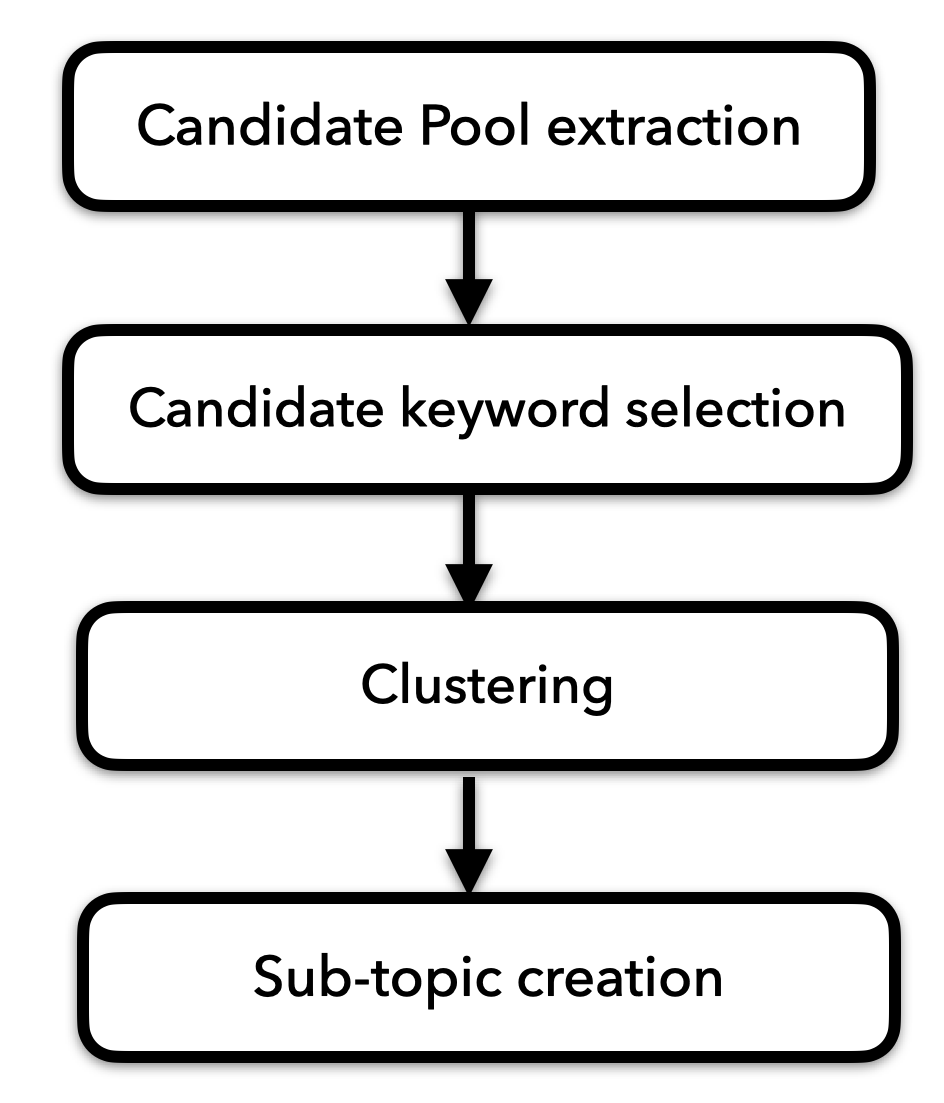
\includegraphics[width=.35\textwidth]{images/thesis_images/methodology.png}
	\caption{Proposed approach on an abstract level. \label{fig:methodology2}}
\end{figure}

The proposed approach, shown in \prettyref{fig:methodology2}, does not assume fixed templates or specific user intentions. The major components in the pipeline are: \emph{Candidate pool selection, Noun-chunk extraction, Automatic keyword extraction, Candidate keyword selection, Clustering, and Sub-topic creation}. The first step of this pipeline is to retrieve a candidate or retrieval pool for the given query. Subsequently, a candidate selection module is proposed to extract keywords with high diversity and low noise (stopwords). This component consists of three significant steps, namely \emph{Noun-chunk extraction, Automatic keyword extraction, and Candidate keyword selection}. Automatic keyword extraction involves extracting the most meaningful noun phrases in a text document. Specific keywords are selected and used for clustering using a percentile selection technique. This process is referred to as candidate keyword selection, and the resulting phrases after this stage are called candidate keywords. The following sections provide a detailed explanation of the above pipeline.




\section{Candidate Pool Selection}


A large set of retrieved documents for the query is required for a wide variety of these sub-topics. This set is referred to as the \emph{Candidate pool} and comprises retrieved results from both semantic and lexical matching. \prettyref{fig:candidate_pool} depicts the generation of the candidate pool from the document indices. A diverse and large candidate pool is crucial for generating a wide variety of query-related sub-topics. The length of a candidate pool directly influences the output of sub-topics, and two candidate pools of lengths around 30 and 100 are considered in this approach. These document pools are constructed from an equal mixture of documents retrieved from lexical and semantic matching.


\begin{figure}[h]
	\centering
	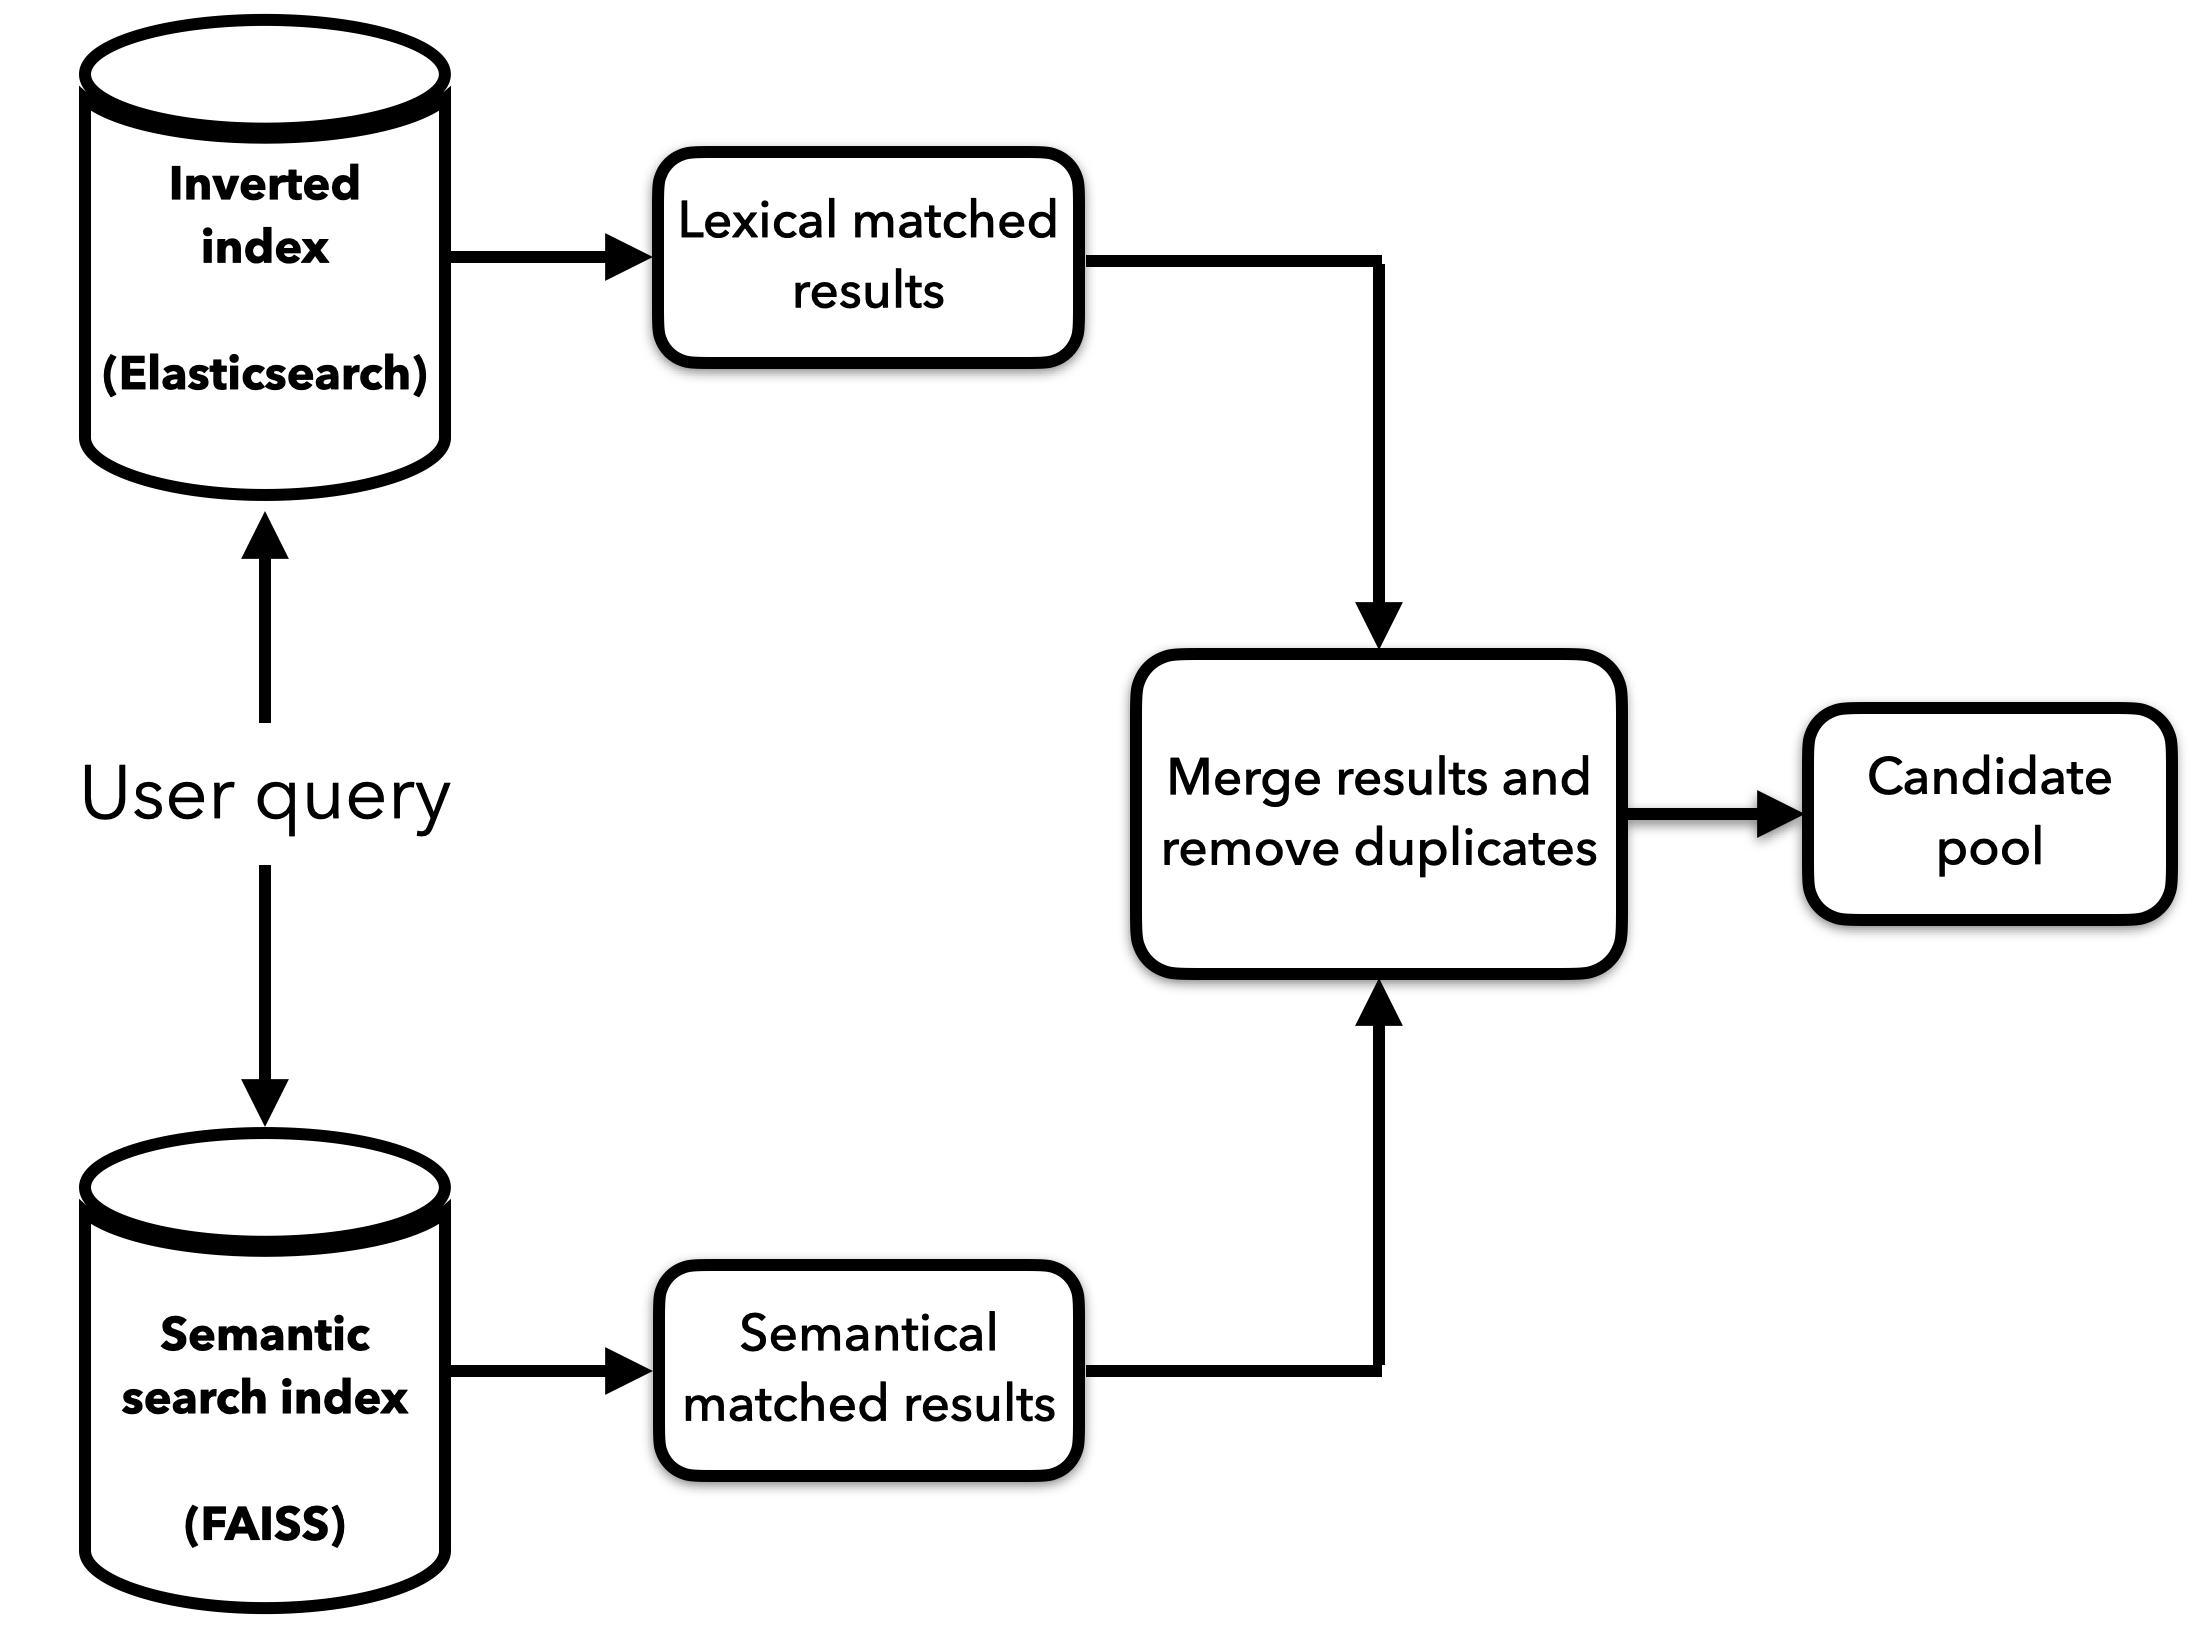
\includegraphics[width=.8\textwidth]{images/thesis_images/candidate_pool.png}
	\caption{Steps to generate a diverse candidate document pool.  \label{fig:candidate_pool}}
\end{figure}

\mycomment{\begin{algorithm}[H]
		\SetKwInput{KwInput}{Input}                % Set the Input
		\SetKwInput{KwOutput}{Output}              % set the Output
		\DontPrintSemicolon
		
		\KwInput{query - string, pool\_size - integer}
		\KwOutput{candidate\_pool - list $[candidate\_pool\_i]$, $i=1, 2, \cdots, n$, where each element is a string}
		% \KwData{Testing set $x$}
		
		% Set Function Names
		\SetKwFunction{FGetcandidate}{Get\_candidate\_pool}
		
		
		% Write Function with word ``Function''
		\SetKwProg{Fn}{Function}{:}{}
		\Fn{\FGetcandidate{$query$, $pool\_size$}}{
			
			\;
			pool\_size\_half = int(pool\_size/2)\;
			\;
			
			\tcc{get\_elastic\_search\_results -  retrieves documents which have high lexical similarity with the query.}
			
			top\_docs\_lexical = get\_elastic\_search\_results (query,  pool\_size\_half)\;
			
			\;
			\tcc{get\_semantic\_matching\_results - retrieves documents which have high semantic similarity with the query.}
			
			top\_docs\_semantic = get\_semantic\_matching\_results (query,  pool\_size\_half)\;
			\;
			
			\tcc{removes common documents which are present in both sets}
			candidate\_pool = remove\_duplicates (top\_docs\_lexical + top\_docs\_semantic)\;
			\;
			
			\KwRet candidate\_pool\;
		}
		\caption{Generate candidate document pool.}
\end{algorithm}}

It is assumed that the top retrieved documents are relevant to the query and the user, and thus, these retrieved documents are used for sub-topic extraction. This assumption can lead to poor sub-topics when the retrieved documents are entirely unrelated to the query, especially in the case of semantic matching. In lexical matching, the retrieved documents contain the query keywords and ensure that the documents are at least partially relevant. However, only cosine similarity is used as the selection criteria in semantic matching. For example, to create a \textit{\ac{CP} of 30} (\ac{CP}-30), top 15 documents from lexical matching results and top 15 documents from semantic matching results are combined. There is a clear possibility that top semantically matched results are not entirely related to the user-given query. Consequently, the cosine similarity of these top semantically matched results needs to be evaluated before creating the candidate pool.

 
 \begin{figure}[h]
 	\centering
 	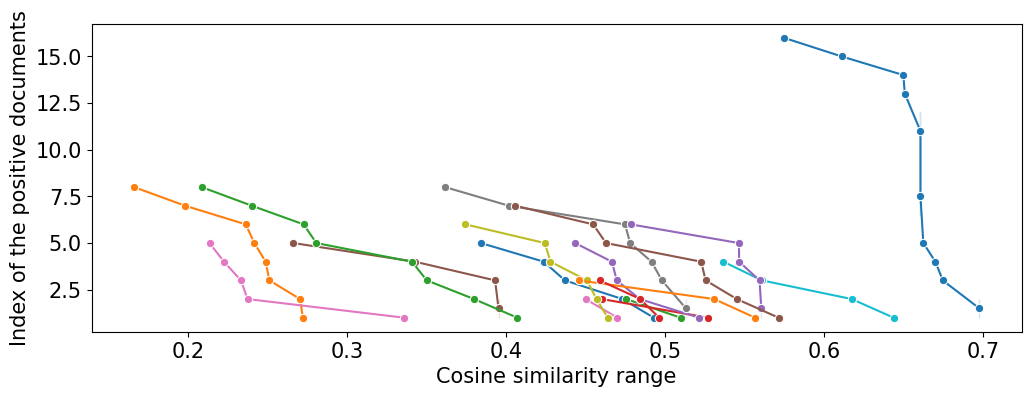
\includegraphics[width=.95\textwidth]{images/results/candidate_pool_analysis.png}
 	\caption[Cosine similarity distribution.]{Cosine similarity between the query and retrieved documents. \label{fig:cosine_sim_range}}
 \end{figure}
 
The cosine similarities between the query and retrieved documents are closely observed to perform this analysis. In the retrieved documents, only relevant documents and the document with the highest cosine similarity are considered. In \prettyref{fig:cosine_sim_range}, each query is shown in a unique colored plot, and it is clear that the spread of cosine similarity differs from query to query. Queries have high cosine similarities with the retrieved results ranging from 0.5, and some queries even have a range up to 0.7. On the other hand, there are some queries with a cosine similarity range below 0.3. Considering the maximum \emph{\ac{CS}} in the retrieved documents ($CS_{\mathrm{max}}$) as the reference, an appropriate lower similarity threshold ($CS_{\mathrm{min}}$) needs to be determined so that only an optimal set of retrieved documents is selected for the candidate pool. This information is represented in the equation below with the help of a cutoff parameter $cp$.
 \\
 
 	\centerline{$CS_{\mathrm{min}}$ = $( cp * CS_{\mathrm{max}} )$}
 	
 	
From the above equation, the value of $cp$ can be determined in multiple ways. One approach tested in this master thesis is the average min-max similarity ratio. The ratio is calculated from the mean of the minimum to maximum cosine similarities over multiple queries. Let us consider the maximum cosine similarity in the retrieved results set of query $q$ as $ max_{\mathrm{q}}$, and the minimum cosine similarity of the relevant document as $ min_{\mathrm{q}}$. Now the approximation of the value $cp$ over $N$ queries is described as:

 
  	\centerline{$cp$ = $( \sum\limits_{q=1}^N  min_{\mathrm{q}}/ max_{\mathrm{q}}) /N$}
 
Applying the above approximation to the data from \prettyref{fig:cosine_sim_range} resulted in the value of $cp$ = 0.78. However, a slightly lower value of 0.75 is chosen in the end, as there may be an expected human bias during data labeling. Multiple labelers are involved in labeling the documents for different queries, and this can lead to possible deviation from the true value. This optimal threshold selection is designed to prevent the selection of irrelevant documents for a given user query. This selection technique can be employed in any semantic matching \ac{IR}.

 

\begin{algorithm}[H]
	\SetKwInput{KwInput}{Input}                % Set the Input
	\SetKwInput{KwOutput}{Output}              % set the Output
	\DontPrintSemicolon
	
	\KwInput{query - string, pool\_size - integer}
	\KwOutput{top\_docs\_semantic - list $[top\_docs\_semantic\_i]$, $i=1, 2, \cdots, n$, where each element is a string}
	% \KwData{Testing set $x$}
	
	% Set Function Names

	\SetKwFunction{FGetsemantic}{Get\_semantic\_matching\_results}
	
	
	% Write Function with word ``Function''
	\SetKwProg{Fn}{Function}{:}{}
	\Fn{\FGetsemantic{$query$, $pool\_size$}}{
		\;
		MIN\_THRESHOLD\_SEMANTIC = 0.27\;
		CP = 0.75\;
		\;
		
		\tcc{top\_docs\_semantic\_search - contains semantically similar documents, doc\_sim\_list - contains respective cosine similarity score}
		
		top\_docs\_semantic\_search, doc\_sim\_list = get\_semantic\_search\_results (query, pool\_size)\;
		\;
		max\_cosine\_sim = max (doc\_sim\_list)\;
		min\_cosine\_sim = min (doc\_sim\_list)\;
		max\_diff\_cosine\_sim = get\_max\_diff\_sim (doc\_sim\_list)\;

		\;
		\tcc{Optimal cutoff similarity selection from three individual cutoffs}
		final\_cutoff\_sim = min (MIN\_THRESHOLD\_SEMANTIC, (CP * max\_cosine\_sim), max\_diff\_cosine\_sim)\;
		\;
		
		top\_docs\_semantic = []\;
		
		
		\For{$idx\gets0$ \KwTo $pool\_size$}{
			\;
			doc = top\_docs\_semantic\_search[$idx$]\;
			sim = doc\_sim\_list[$idx$]\;
			
			\tcp{Selecting documents that have high cosine similarty than the optimal cutoff similarity.}
			\If{sim > final\_cutoff\_sim}
			{
				top\_document\_semantic.append(doc)\;
			}

		}
		\;
		
		
		\If{len (top\_docs\_semantic) < 10}
		{
			\tcc{Selecting only top 10 in case of poor similarity distribution between the query and documents}
		top\_docs\_semantic = top\_docs\_semantic\_search[:10]\;
		}
		\;

		 	\caption{Retrieve semantically similar documents with optimal selection.} \label{algo:optimal_selection}
		\KwRet top\_docs\_semantic\;
	}
	
\end{algorithm}


Furthermore, it is also observed that some queries exhibit abnormal cosine similarity distributions, such as cosine similarity values below 0.3 as shown in \prettyref{fig:cosine_sim_range}. An optimal candidate pool selection approach is proposed to handle these exceptional cases. This technique extends the existing threshold by considering two additional criteria. These criteria are chosen in the context of unexpected or poor query-to-document distributions. The first criterion establishes a fixed threshold for cosine similarity, while the second criterion captures the maximum difference in cosine similarity between the top two similar documents.

 Algorithms \prettyref{algo:optimal_selection} and \prettyref{algo:max_diff} further detail these criteria. In the case of no results at the end of the selection, the top 10 semantically matched documents are chosen. After the successful selection of documents from semantic matching, the documents from lexical matching are combined and duplicates are removed. The resulting set of documents without any redundancy is then referred to as the candidate pool.

 
 \begin{algorithm}[H]
 	\SetKwInput{KwInput}{Input}                % Set the Input
 	\SetKwInput{KwOutput}{Output}              % set the Output
 	\DontPrintSemicolon
 	
 	\KwInput{sim\_list - list $[sim\_list\_i]$, $i=1, 2, \cdots, n$, where each element is a float }
 	\KwOutput{max\_diff\_sim - float}
 	% \KwData{Testing set $x$}
 	
 	% Set Function Names
 	\SetKwFunction{FMaxdiffsim}{Get\_max\_diff\_sim}
 	
 	% Write Function with word ``Function''
 	\SetKwProg{Fn}{Function}{:}{}
 	\Fn{\FMaxdiffsim{$sim\_list$}}{
 		
 		\;
 		diff\_list = []\;
 		sim\_list\_len = len(sim\_list)\;
 		\;
 		
 		\For{$idx\gets1$ \KwTo $sim\_list\_len$}{
 			\tcp{store the difference in similarities at recurrent indices.}
 			diff\_list.append(sim\_list [$idx$] - sim\_list [$idx$ - 1])
 		}
 		\;
 		
 		max\_diff = max(diff\_list)\;
 		\tcp{Get the index where the similarity difference is maximum.}
 		max\_diff\_index =  diff\_list.index(max\_diff)\;
 		\;
 		
 		max\_diff\_sim = sim\_list[max\_diff\_index]\;
 		\;
 		\KwRet max\_diff\_sim\;
 	}
 	
 	\caption{Calculate similarity at the maximum difference.} \label{algo:max_diff}
 \end{algorithm}

\section{Candidate Keyword Selection}

This section details the steps involved in selecting specific keywords and the criteria involved
in their selection. The main objective of this stage is to choose highly diverse noun chunks from each
text document. Candidate keyword selection is the most crucial step in the entire pipeline, and the
quality of the clustering output directly depends on the outcome of this step.

\subsection{Noun Chunk Extraction}

News-articles are very long text documents and nouns serve as essential parts of speech elements that identify people, places, or things. A noun chunk is a phrase (a group of words) that represents a noun. To automatically extract the noun chunks from each document, a library named \emph{spacy}\footnote{\url{https://spacy.io/}} is used. The noun chunks from spacy are closely analyzed, and some inconsistencies are identified that require further cleaning. A unique pipeline is proposed to clean these noun chunks, targeting the noise elements: stopwords, punctuation, determiners, duplicates, and long noun chunks.

 
 \begin{description}
 	\item[Remove longer Noun-chunks] \hfill \\  It has been observed in the output of spacy noun chunks that there are some  noun phrases consisting of more than three words, which mostly lack significant information. Consequently, these noun chunks are removed from the spacy output. For example, in German, the phrase \emph{"standort- und zeitunabhängigen Zusammenarbeit"} and in English, the phrase \emph{"Every successive cellular generation"}. Although there might be useful information within these long noun phrases, extracting that information is very challenging. The occurrence ratio of these phrases is relatively smaller compared to phrases with a length below 3. Therefore, these long noun phrases are filtered out from the set of noun chunks.
 	
 	\item[Remove stopwords] \hfill \\  Stopwords are words that carry no significant information and are thus omitted from the noun chunks. There is no universal set of stopwords in any language, and there are also numerous types of stopwords observed in news-articles in both English and German languages. Therefore, a robust set of stopwords from various sources\footnote{\url{https://gist.github.com/sebleier/554280, https://countwordsfree.com/stopwords, https://solariz.de/de/downloads/6/german-enhanced-stopwords.htm}} has been collected in both languages. Stopwords can appear either as a complete noun chunk or as part of a noun chunk, and they are removed in either case. Stopwords generally consist of determiners, adjectives, articles, prepositions, etc.
 	
 	
 	\item[Remove numeric noun chunks] \hfill \\  Some noun chunks have numeric values that contain no useful information, and furthermore, it is observed that the complete noun chunk does not convey any significance either. Thus, the numeric noun chunks are removed from the noun chunks set. For example, \emph{"mehr als 50 Ländern", "1,95 m Länge", "1,5 Milliarden"} in German, etc. However, the noun chunks where the numeric value is attached to an alphabet are ignored, i.e., \emph{"4G Technology", "3D designs"} in English, etc.
 	
 	
 	\item[Remove punctuation]  \hfill \\ This step is designed to remove all sorts of punctuation elements and keep the noun chunks clean and more readable to the user. For example, the original noun chunk "Bündnis- und Landesverteidigung" is transformed to \emph{"Bündnis Landesverteidigung"} after removing the hyphen (-) and the stopword (und).
 	
 	
 	\item[Lemmatization] \hfill \\  Lemmatization is the process of extracting the base or normalized form from the original words~\cite{plisson2004rule}. For example, 'worse' and 'worst' are lemmatized to their base form 'bad'. Lemmatization helps text processing techniques based on lexical matching and reduces computational and storage complexity. In this thesis, lemmatization is performed with the help of spacy library for both the English and German languages.
 	
 	
 	\item[Fuzzy redundancy removal] \hfill \\  It is observed that there are a lot of noun chunks that are syntactically similar to each other. These similar noun chunks can be categorized into two types, namely exact duplicates and close duplicates. Exact duplicate noun chunks can be easily filtered in Python, but identifying the close duplicates and filtering is a challenge. For example, the noun chunks "5G network" and "5G 4G network". 
 	
 	Only one of the noun chunks i.e. longer noun chunk is retained, and the other is removed. Algorithm \prettyref{algo:close_duplicates} details the steps used to achieve the cleaned noun chunks. The main objective of this step is to reduce the similar phrases and increase diversity in the data. This can lead to a loss of information to a certain extent. Accordingly, a fuzzy string matching-based noun chunk removal approach is designed to tackle the above problem, and close duplicates are removed to a certain extent using the FuzzyWuzzy library (refer to Appendix \ref{appendix:A} for more information).
 	
 	
 \end{description}

 	
 	\begin{algorithm}[H]
	\SetKwInput{KwInput}{Input}                % Set the Input
	\SetKwInput{KwOutput}{Output}              % set the Output
	\DontPrintSemicolon
	
	\KwInput{noun\_chunk\_list - list $[noun\_chunk\_list\_i]$, $i=1, 2, \cdots, n$, where each element is a string }
	\KwOutput{cleaned\_noun\_chunk\_list - list $[cleaned\_noun\_chunk\_list\_i]$, $i=1, 2, \cdots, n$, where each element is a string }
	% \KwData{Testing set $x$}
	
	% Set Function Names
	\SetKwFunction{FRemovdup}{Remove\_close\_duplicates}
	
	% Write Function with word ``Function''
	\SetKwProg{Fn}{Function}{:}{}
	\Fn{\FRemovdup{$noun\_chunk\_list$}}{
		
		\;
		\tcp{Removing exact duplicates using set in python}
		noun\_chunk\_list = list(set(noun\_chunk\_list))\;
		
		
		\;
		close\_duplicates = []\;
		noun\_chunk\_list\_len = len(noun\_chunk\_list)\;
		
		\;
		
		\For{$i\gets1$ \KwTo $noun\_chunk\_list\_len$}{
			
			phrase\_1 = noun\_chunk\_list [$i$]\;
			\;
			
			\For{$j\gets i+1$ \KwTo $noun\_chunk\_list\_len$}{
				
				phrase\_2 = noun\_chunk\_list [$j$]\;
				\;
				
				\tcp{fuzzy gives the syntactical text similarity score}
				\If{fuzzy (phrase\_1, phrase\_2) > 85}
				{
					
					\tcp{When the score is high, the smaller phrase is recorded}
					
					close\_duplicates.append(get\_shorter\_text(phrase\_1, phrase\_2))\;
				}
				\;
				
				
			}
			\;
			
		}
		\;
		
		\tcp{Removing the close duplicates using recorded close\_duplicates}
		cleaned\_noun\_chunk\_list = list(set(noun\_chunk\_list) - set(close\_duplicates))\;
		\;
		\KwRet cleaned\_noun\_chunk\_list\;
	}
	
	\caption{Algorithm to remove close duplicates.} \label{algo:close_duplicates}
\end{algorithm}


\subsection{Keyword Extraction}
The cleaned noun chunks describe a text document very well. However, not all noun chunks are of great significance in representing a document, especially in the case of a news-article. As the length of the news article is large, the size of the extracted noun chunk set can also be large. This large set of noun chunks is well-processed syntactically. It needs to be processed now semantically to select only noun chunks that can significantly influence the meaning of a text document (a news article). These crucial noun chunks in a text document are referred to as \textit{Keywords}.


Transformer architectures compute context-aware embeddings of tokens in a sentence, considering the order and identity of the tokens. These token-level representations are further averaged to calculate sentence embeddings. However, using sentence-level embeddings as the mean of token embeddings can result in poor representations of long text documents. In news articles, it is observed that the length of the text documents is longer, and different contexts are discussed in different paragraphs. Therefore, the document is divided into multiple paragraphs, and the mean of all paragraph embeddings is considered as a "Document representation vector". In this approach, a paragraph length of 500 tokens is considered. For example, a text document with a token length of 1600 is divided into four paragraphs of lengths 500, 500, 500, and 100, respectively. The final document representation vector is the mean representation vector of these paragraph vectors. The best possible parameter for the paragraph length is not explicitly tested in this master thesis and can be considered as future work.



\begin{figure}[h]
	\centering
	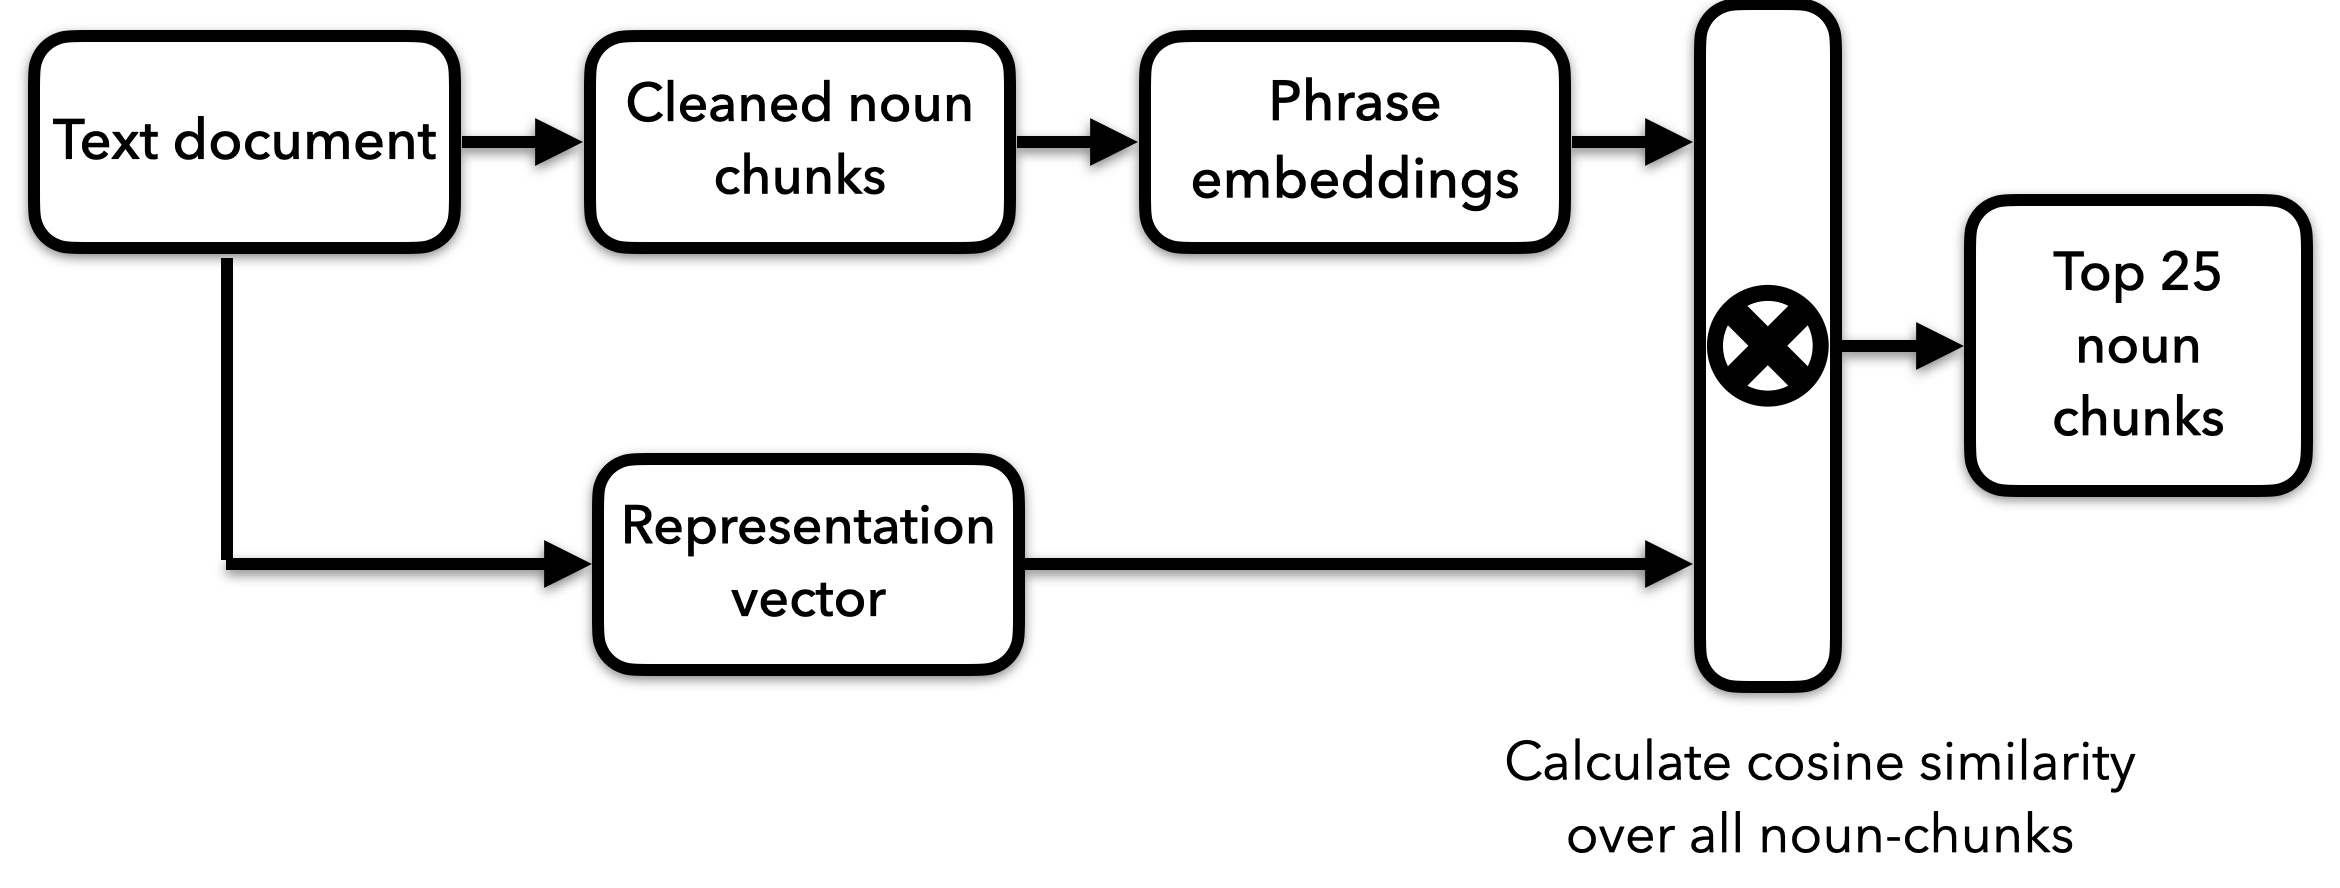
\includegraphics[width=.9\textwidth]{images/thesis_images/keyword_extraction.png}
	\caption[Contextualized automatic keyword extraction.]{Automatic keyword extraction using phrase embeddings. \label{fig:keyword_extraction}}
\end{figure}


Phrase embeddings are semantic representations of noun chunks that are computed using the \ac{USE} model. By utilizing noun chunk embeddings and the document representation vector, the relevance of a noun chunk in a document is expressed as the cosine similarity between the vectors in the semantic space. The higher the similarity, the greater the relevance of the noun chunk in the document. Consequently, all noun chunks are ranked according to their similarity of relevance with the document. The top 25 noun chunks with the highest relevance similarity are considered as "Keywords". The pipeline for extracting these keywords is shown in \prettyref{fig:keyword_extraction}.


\subsection{Candidate Keyword Selection}


Keywords extracted from a document in the earlier stage are syntactically diverse, as they are derived from the noun chunks generated by removing the close duplicates. Let us consider the case of using these keywords to distinguish documents in an \ac{IR} setup, where the user provides a search query and expects relevant documents. Through preliminary manual analysis, it has been observed that there are certain keywords that are dissimilar to the user query but hold significant value in improving the information search behavior. Therefore, the task of removing the query-related keywords and retaining the highly distinctive keywords is referred to as \emph{Candidate keyword selection}.


Let us consider a text corpus $C$ that contains $n$ documents, where each document $D$ is a news article. These documents are stored in two indices, namely the inverted index and the semantic search indices, for retrieving documents based on a given search query.


\centerline{$C$ = $\{D_1, D_2, D_3,\dots, D_n\}$}

Once the user provides the IR system a search query $q$ and a candidate pool $CP$ of size $m$ is generated, which is a document set.

\centerline{$CP_q$ = $\{D_i, D_j, D_k,\dots\}$}


Taking one document $D_i$ into account, a set of keywords ($k$) is extracted using the above steps, namely noun chunking and automatic keyword extraction. The news-article is then transformed into a group of keywords, as expressed below.


\centerline{$D_i$ = $\{k_1, k_2, k_3,\dots\}$ } 

The objective of this step is to efficiently select specific keywords that are similar to the query. This selection process also takes into consideration the close semantic and multi-lingual nature of the keywords. To achieve this, cosine similarity is utilized, and the multi-lingual \ac{USE} model is employed to encode both the query and the keywords into semantic embeddings. The similarity between the query and the document keywords is determined by the distance in the semantic space. Keywords with low cosine similarity are selected to ensure a diverse range of keywords in relation to the query. To remove keywords that are similar to the query, a parameter called candidate keyword selection ($cks$) parameter is proposed.

The selection parameter considers the distribution of similarity between the query and keywords within a document. Furthermore, it should be independent of any specific document. A percentile selection criterion is adopted to avoid using a static similarity threshold. The similarity score of the $x$ percentile indicates that the score is higher than $x$ percent of the population or the similarity is lower than $100-x$ percent of the population. In the case of $cks$-based selection, only the keywords that are not similar to the query are of interest, and are therefore selected. For example, $cks$ = 60 denotes the selection of keywords with query similarity less than the 60th percentile similarity and the removal of keywords higher than the 60th percentile. Similarly, a value of $cks$ = 100 represents the selection of all keywords without any removal. 

The keywords selected as the outcome of candidate keyword selection are referred to as "Candidate keywords". After candidate keyword selection process for a given user query $q$, one document  or news-article $D_i$ can be represented as a set of candidate keywords $ck$. Notably, candidate keywords are a subset of keywords.


\centerline{$D_i$ = $\{ck_1, ck_2, ck_3,\dots\}$ } 


The keyword selection for a given $cks$ parameter is illustrated in \prettyref{tab:cks_selection}. As far as my knowledge goes, this selective approach to improving clustering and \ac{IR} performance is one of the earliest attempts in \ac{IR} system research. Additional criteria for enhanced keyword selection, beyond query similarity, should be further explored in the future work.

\begin{center}
	\captionof{table}{Different $cks$ parameter examples.}\label{tab:cks_selection}
	\begin{tabularx}{.9\textwidth}{|c|Y|}
		\hline
		Cks parameter  &  Selected candidate keywords  \\
		\hline
		
		\textbf{100}  &            All keywords are selected   \\ \hline
		75 &            Keywords with query similarity lower than 75th percentile  \\ \hline
		50 &            Keywords with query similarity lower than 50th percentile  \\ \hline
		25 &            Keywords with query similarity lower than 25th percentile   \\ \hline
		10 &            Keywords with query similarity lower than 10th percentile \\ \hline
		
	\end{tabularx}
	
\end{center}



\section{Keyword Clustering}

Candidate keywords from each document in the candidate pool are combined, and duplicates are removed to create a final set of candidate keywords. The combined candidate keywords set from all news-articles in the candidate pool for a query $q$ is represented as $M_q$. These keywords are further clustered using the \ac{HDBSCAN} algorithm to generate distinctive sub-topics. This stage has three main steps, namely \emph{Phrase embeddings extraction}, \emph{Dimensionality reduction}, and \emph{Hierarchical clustering}. 

To achieve semantic clustering, multi-lingual \ac{USE} model are used to generate phrase embeddings for each candidate keyword. These densely distributed embeddings are usually highly dimensional (512), and clustering in high-dimensional space is complex to capture patterns and can be resource-intensive. Therefore, the embeddings are compressed with the help of a dimensionality reduction technique, namely \ac{UMAP}. The dimensionality of the embeddings is reduced without losing underlying information in the data using the \ac{UMAP} algorithm~\cite{mcinnes2018umap} from the umap-learn\footnote{\url{https://pypi.org/project/umap-learn/}} library.

\begin{figure}[h]
	\centering
	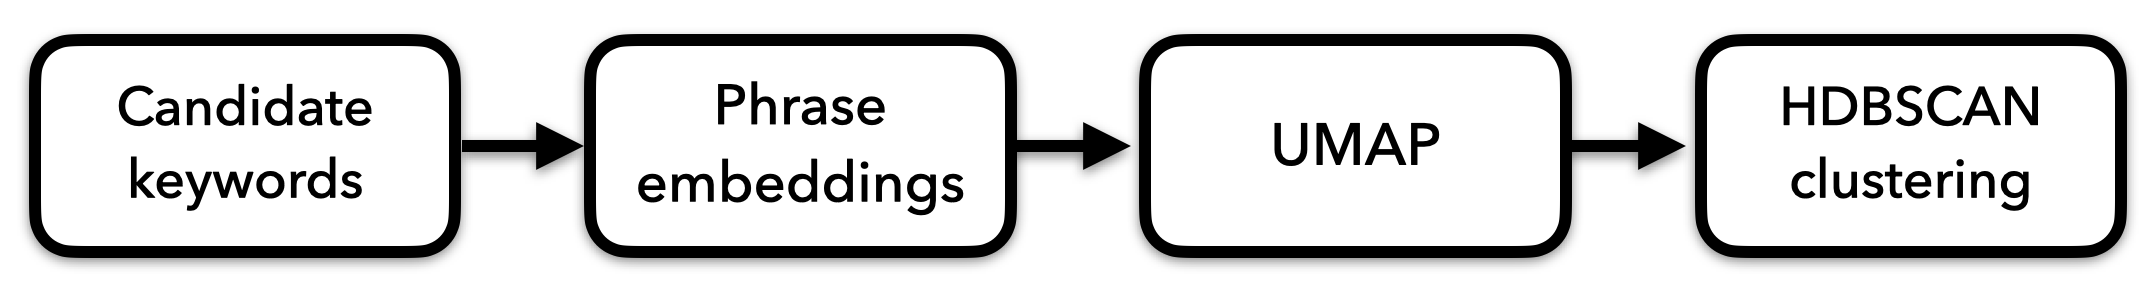
\includegraphics[width=.9\textwidth]{images/thesis_images/clustering.png}
	\caption{Clustering to generate sub-topics.  \label{fig:clustering}}
\end{figure}

 
These embeddings are further clustered in low dimensions using a hierarchical clustering algorithm. Noise is expected in the candidate keyword extraction phase, and not all keywords are crucial for modeling. Therefore, clustering algorithms such as k-means and gaussian mixture models are not suggested in this case, as they assign all data points to a cluster during clustering. Furthermore, these algorithms assume a specific cluster shape, either spherical or elliptical. Consequently, density-based algorithms like the \ac{HDBSCAN} clustering algorithm are preferred because they inherently account for noise in the data and prevent assigning a cluster to every data point.

One significant advantage of these algorithms is that the number of clusters is not a parameter, and the algorithm effectively creates clusters based on the data. The \ac{HDBSCAN} algorithm~\cite{mcinnes2017hdbscan}, with its varying epsilon and merging clusters, has shown robust clustering results by finding clusters with varying densities. The same algorithm is considered in this master's thesis. \prettyref{fig:clustering} presents the steps taken to perform clustering after extracting the candidate keywords. This clustering pipeline has already been tested and has shown excellent results with documents in recent research~\cite{angelov2020top2vec}. However, in this approach, keywords are clustered rather than the documents, and later the keywords and documents are connected using "sub-topics".




\section{Sub-topic Creation} 

After clustering, sub-topics are extracted using a centroid approach. A mean phrase vector (centroid vector) is calculated from all the keywords inside a cluster, and the closest keyword vector to the centroid vector is considered a cluster label. This process is named \textit{Cluster labeling}, and the cluster labels are considered as "Sub-topics". Sub-topics and documents inside a sub-topic can be further ranked before showing them to the user. The pipeline ends with this last component, \emph{Sub-topic creation}.  The phrases "sub-topic modeling" or "sub-topic clustering" are identical to the outcome of complete pipeline. The code developed for the complete sub-topic retrieval and testing is shared in the GitHub repository \textit{Sub-topic-retrieval-thesis}\footnote{\url{https://github.com/praveengadiyaram369/Sub-topic-retrieval-thesis}}.


Thereafter the candidate keyword set $M_q$ is clustered into $r$ groups ($s$) and is defined as a sub-topic set $S_q$. 

\centerline{$S_q$ = $\{s_i, s_j, s_k,\dots, s_r\}$}

Each sub-topic ($s$) is again expressed as a set of candidate keywords  ($ck$). The number of candidate keywords in a sub-topic cluster can vary from cluster to cluster.

\centerline{$s_i$ = $\{ck_x, ck_y, ck_z,\dots\}$}

The mapping between the document and keywords has already been established above. Now, each document can be expressed as a set of sub-topics, where each sub-topic is further described as a set of documents. Candidate keywords serve as the foundational concepts for the modeling relationship between the sub-topics and documents.

\centerline{$D_p$ = $\{s_i, s_j, s_k,\dots\}$ }
\centerline{$s_q$ = $\{D_x, D_y, D_z,\dots\}$}


